\documentclass[12pt,english]{rftthesis}

\usepackage[utf8]{inputenc}
\usepackage[T1]{fontenc}
\usepackage{csquotes}
\usepackage{graphicx}
\usepackage{setspace}
\usepackage{wrapfig}
\usepackage{float}

\setacronymstyle{long-short}


\title           {Development of snapshot and fault injection techniques within Dream Chaser's COMS system's hypervisor}
\type            {Masters thesis abstract}
\author          {B.Eng. Alexis Cabana-Loriaux}
\matriculation   {0407200}
\studies         {Masters of Space Engineering}
\firstsupervisor {Prof. Dr.-Ing. Klaus Brieß}
\secondsupervisor{Dipl.-Ing. XXXX}
\industrysupervisor{Dipl.-Ing. Claudio Discepola}
\date            {\today}

\begin{document}
\onehalfspacing

%
%  HEADER
%
\begin{center}
\begin{large}
Project description - Masters thesis
\end{large}
\\
\vspace{.5cm}
\begin{LARGE}
Development of Snapshot and Fault Injection Techniques within Dream Chaser's Software-in-the-loop Test Framework
\end{LARGE}
\end{center}

%
%  Intro 
%
\section*{Introduction}\label{sec:intro}
The Dream Chaser Cargo System (DCCS) is a reusable orbital spaceplane from Sierra Nevada Corporation (SNC) intented for the resupply of both pressurized and unpressurized cargo to the International Space Station. The vehicle, whose development started in 2010, is to be launched on United Launch Alliance rockets, with the possibility of also serving european interests in space in the future. Since then, SNC has put MacDonald, Dettwiler and Associates Ltd. (MDA) in charge of the systems engineering and the development of the communication subsytem of DCCS. MDA is the industry supporter of the present thesis.

\begin{wrapfigure}{R}{0.45\textwidth}
\centering
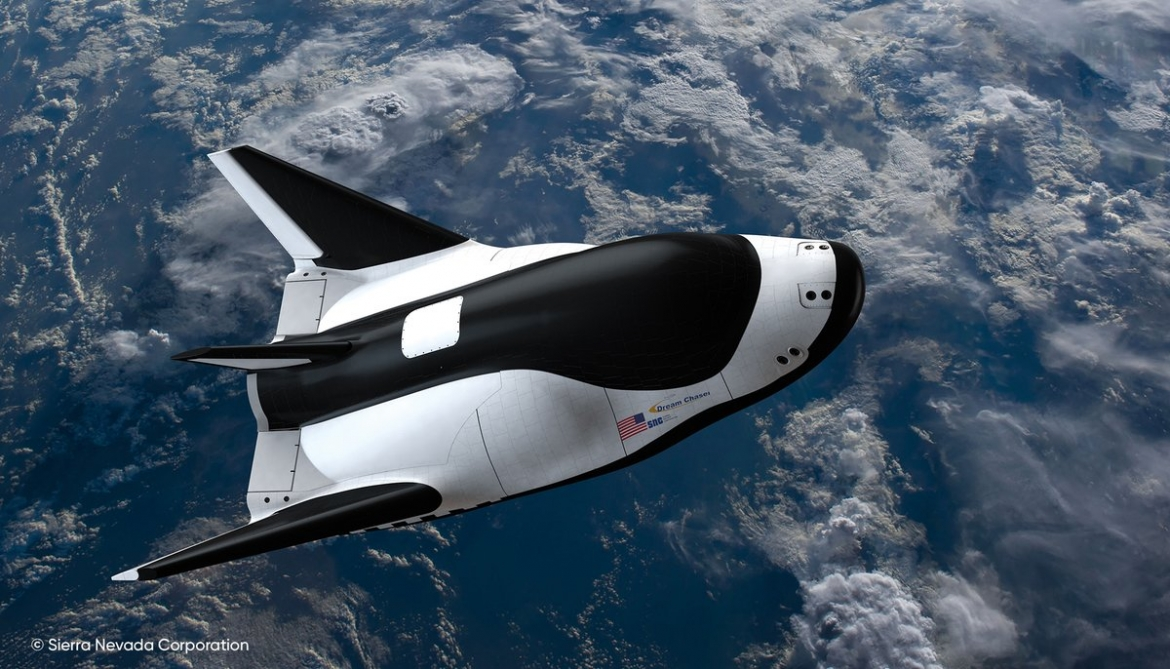
\includegraphics[width=0.43\textwidth]{art/dccs}
\caption{\label{fig:dccs}Artist impression of the Dream Chaser Cargo System. [Sierra Nevada Corporation]}
\end{wrapfigure}

With the ever decreasing cost of computing power, functional simulation of components and systems has become an integral part of the testing phase in space design. This approach is thus also taken by SNC, who requires their technology partners like MDA to provide simulators of their respective subsystems in order to mimic the behavior of some segments of the spacecraft in action together. As such, MDA is developing the Baseband Processor Simulator (BBPSim), a hypervisor that runs the COMS subsystem's software.

%
%  Purpose 
%
\section*{Purpose}\label{sec:purpose}
The present Thesis shall firstly analyze different \textit{snapshotting} strategies of the DCCS Application Software (DAS) within the BBPSim simulator. This technique will enable saving the running state of DAS, storing it in non-volatile memory and restoring DAS to a past saved state. \textit{Snapshotting} is a highly desirable feature that enables rerun of integration tests under the same conditions. An exhaustive research shall be conducted on similar existing solutions, notably in virtual machine software and in the Linux kernel. An adapted solution will then be designed and implemented to fit BBPSim. 

Secondly, the Thesis will investigate various existing fault injection techniques, both in hardware and software, in order to develop and incorporate a custom-fit, software-in-the-loop solution in BBPSim. Fault injection will allow testing DAS to guarantee it can recover from error conditions.
%
%  Tasks 
%
\section*{Summary of tasks}\label{sec:tasks}
\begin{itemize}
\item Litterature research on the various state snapshotting/storing and fault injection methods, both in existing software and in a self-developed approach
\item Identify usable concepts in the context of BBPSim and how they can adapt to fit MDA's needs 
\item Design a custom solution for non-intrusive snapshotting, state representation/storage/recovery and fault injection testing process, then integrate it in BBPSim
\item Implement and document the chosen concepts in software
\item Validate workability from a user's perspective
\item Assess the impact on the existing testing pipeline of DAS and on its long-term robustness
\end{itemize}

\subsection*{Supervisor}
\begin{spacing}{1}
Claudio Discepola\\
Senior Member, Technical Staff\\
+1-514-457-2150, Ext. 3170\\
claudio.discepola@mdacorporation.com
\end{spacing}

\begin{figure}[H]
	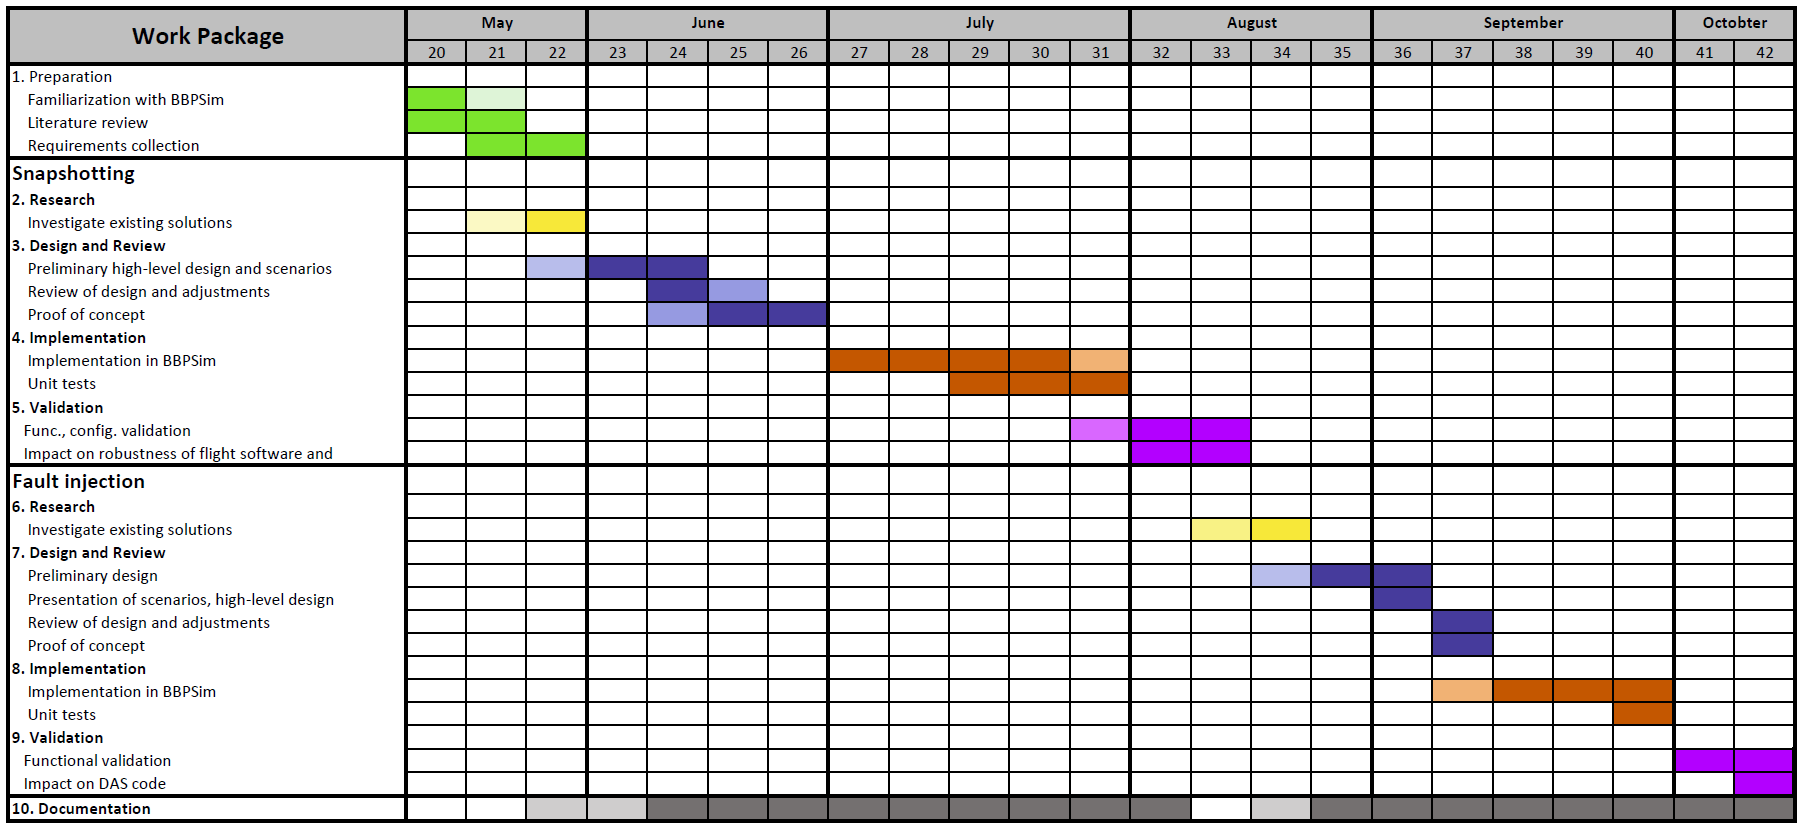
\includegraphics[scale=0.3]{art/time_plan.png}
	\caption{Thesis time plan}
\end{figure}

\end{document}
